\section{Convolution}
In this lecture we are going to deal with the topic of convolution. The general definition is given by:
\[
    (f*g)(x) = \int_{-\infty}^{+\infty} f(t)g(x-t)dt    
\]
The operation can be applied also to vector with:
\[
    (\underline{c}*\underline{d})_K = \sum_{i+j = k} c_i d_j = \sum_i c_i d_{k-i}    
\]
The pedix $K$ is used to indicate the $k$-th element of the vector to which is the convolution is applied. The vectors can be expressed also as polynomials:
\[
    c(x) = c_0 + c_1 x + c_2 x^2 + \dots + c_{n-1} x^{n-1}    
\]
\[
    d(x) = d_0 + d_1 x + d_2 x^2 + \dots + d_{n-1} x^{n-1}
\]
The convolution is the product of these polynomials. [to finish]


\subsection*{Cyclic convolution}
The cyclic convolution is a particular case of convolution in which the vectors are cyclic. This means that the last element of the vector is followed by the first one. The cyclic convolution is defined as:
\[
    (\underline{c}\circledast \underline{d})_K = \sum_{i+j = k \mod(n)} c_i d_j 
\]
How can this be written in matrix form?
\begin{multicols}{2}
    \begin{center}
        \textsc{Convolution}
    \end{center}
    In this case are used the \textbf{Toeplitz matrices} (or also called Time-Invariant Linear Systems), the elements are given by $(2n - 1)$-length sequence:
    \[
        \left\{t_K: -(n-1) \leq K \leq (n-1) \right\}    
    \]
    The element in position $(i,j)$ is given by $T(i,j) = t_i - t_j$ and the generic Toeplitz matrix as this shape:
\[
T = \begin{bmatrix}
    t_0 & t_1 & t_2 & t_3 \\
    t_{-1} & t_0 & t_1 & t_2 \\
    t_{-2} & t_{-1} & t_0 & t_1 \\
    t_{-3} & t_{-2} & t_{-1} & t_0
\end{bmatrix}
\]
    So, it's easy to notice that on the diagonal there is always a constant vector.
    \newcolumn
    \begin{center}
        \textsc{Cyclic convolution}
    \end{center}
    In this case are used the \textbf{Circulant matrices}, a particular case of a Toeplitz matrix. For a given $n \times n$ matrix, the elements are given by $(n)$-length sequence:
    \[
        \left\{c_K: 0 \leq K \leq (n-1) \right\}
    \]
    The element in position $(i,j)$ is given by $C(i,j) = c_{i-j \mod(n)}$ and the generic Circulant matrix as this shape:
    \[
        C = \begin{bmatrix}
            c_0 & c_{n-1} & c_{n-2} & \dots & c_1 \\
            c_1 & c_0 & c_{n-1} & \dots & c_2 \\
            c_2 & c_1 & c_0 & \dots & c_3 \\
            \vdots & \vdots & \vdots & \ddots & \vdots \\
            c_{n-1} & c_{n-2} & c_{n-3} & \dots & c_0
        \end{bmatrix}
    \]
    As you can see, the last element of a column vector becomes the first element of the next column vector, for this reason is called circulant. 
\end{multicols}
Example of circulant matrix:
\[
    C = \begin{bmatrix}
        1 & 8 & 5 & 3\\
        3 & 1 & 8 & 5\\
        5 & 3 & 1 & 8\\
        8 & 5 & 3 & 1
    \end{bmatrix}    
\]
Now we introduce a \textbf{permutation matrix} $P$ defined as follows:
\[
    P = \begin{bmatrix}
        0 & 1 & 0 & 0\\
        0 & 0 & 1 & 0\\
        0 & 0 & 0 & 1\\
        1 & 0 & 0 & 0
    \end{bmatrix}
\]
If we multiply the permutation matrix with a vector, this happen:
\[
    P \underline{c} = \begin{bmatrix}
        0 & 1 & 0 & 0\\
        0 & 0 & 1 & 0\\
        0 & 0 & 0 & 1\\
        1 & 0 & 0 & 0
    \end{bmatrix} \begin{bmatrix}
        c_0\\
        c_1\\
        c_2\\
        c_3
    \end{bmatrix} = \begin{bmatrix}
        c_1\\
        c_2\\
        c_3\\
        c_0
    \end{bmatrix}    
\]
All elements are shifted of 1 position. This means that the circulant matrix $C$ can be built as follows:
\[
    C = c_0 I + c_1 P + c_2 P^2 + c_3 P^3    
\]
This is true for any circulant matrix so we define also $D$:
\[
    D = d_0 I + d_1 P + d_2 P^2 + d_3 P^3 
\]
What happen when we multiply $CD$, i.e two circulant matrices?
\[
    CD = (c_0 I + c_1 P + c_2 P^2 + c_3 P^3)(d_0 I + d_1 P + d_2 P^2 + d_3 P^3)
\]
But this means that we end up with elements with $P^4$ and $P^5$ and so on, but $P^4 = I$, $P^5 = P$ and $P^6 = P^2$. This makes sense even considering that we are dealing with circulant matrices. In general we can say:
\[
    P_n \text{ of } n \times n \implies P^n = I    
\]


\subsection*{Eigenvectors and eigenvalues of a circuland matrix}
Let's start considering again the permutation matrix $P$. We can compute its eigenvalues by using the definition method:
\[
    P - \lambda I = \begin{bmatrix}
        -\lambda & 1 & 0 & 0\\
        0 & -\lambda & 1 & 0\\
        0 & 0 & -\lambda & 1\\
        1 & 0 & 0 & -\lambda
    \end{bmatrix}
    \implies
    \det(P - \lambda I) = \lambda^4 - 1 = 0
\]

So the eigenvalues of $P$ are the fourth roots of 1, which correspond to:
\begin{multicols}{2}
    \begin{center}
        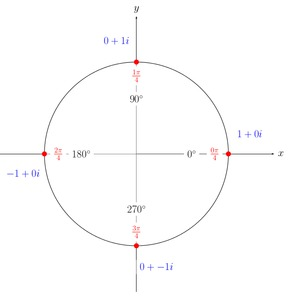
\includegraphics[scale = 0.4]{../images/FourthRoots.jpg}
    \end{center}
    \newcolumn
    \vspace{0.2cm}
    \[
        \begin{split}
            &\lambda^4 - 1 = 0\\
            &\lambda_1 = 1\\
            &\lambda_2 = i\\
            &\lambda_3 = -1\\
            &\lambda_4 = -i
        \end{split}    
    \]
\end{multicols}
We introduce now the complex number $w$ given by:
\[
    w^i = e^{\dfrac{2\pi i}{n}} \overset{\text{in this case}}{\longrightarrow}    w^i = e^{\dfrac{2\pi i}{4}} \implies \begin{cases}
        \lambda_1 = w^0\\
        \lambda_2 = w^1\\
        \lambda_3 = w^2\\
        \lambda_4 = w^3
    \end{cases}
\]
In general we have:
\[
    P_n \implies \lambda^n - 1 = 0 \implies w^0, w^1, \dots, w^{n-1}
\]
Another property of $P$: it's orthogonal indeed $P^\intercal P = I$.
What about the eigenvectors of $P$? Consider the generic matrix $C$ written in terms of $P$:
\[
    C = c_0 I + c_1 P + c_2 P^2 + c_3 P^3    
\]
We want to find the eigenvectors of $C$. If $\lambda_k, \underline{v}_k$ is the couple of eigenvalue and eigenvector of $P$, then:
\[
    \begin{split}
        P\underline{v}_k &= \lambda_k \underline{v}_k\\
        (c_0 I + c_1 P + c_2 P^2 + c_3 P^3)\underline{v}_k &= (c_0 + c_1 \lambda_k + c_2 \lambda_k^2 + c_3 \lambda_k^3)\underline{v}_k\\
    \end{split}
\]
$\underline{v}_k$ is an eigenvector of $C$.\\




\section{Discrete Fourier Transform}

Consider the general theory of eigenvalues and eigenvectors. Given a square matrix \( A \), an eigenvalue \( \lambda \) and an associated eigenvector \( \underline{v} \) are defined such that:
\[
A \underline{v} = \lambda \underline{v}
\]
This implies that the action of the matrix \( A \) on the vector \( \underline{v} \) is equivalent to scaling \( \underline{v} \) by \( \lambda \).

\subsection*{Eigenvalues and Eigenvectors of a Circulant Matrix}
A circulant matrix \( C \) can be defined in terms of its generating vector \( \underline{c} \). The eigenvalues and eigenvectors of \( C \) can be obtained through the Discrete Fourier Transform (DFT). Specifically, if \( \mathbf{F} \) represents the Fourier matrix, then:
\[
C = \mathbf{F}^{-1} \Lambda \mathbf{F}
\]
where \( \Lambda \) is a diagonal matrix containing the eigenvalues of \( C \).

\subsection*{Discrete Fourier Transform (DFT)}
The DFT of a vector \( \underline{c} \) is computed by multiplying it by the Fourier matrix \( \mathbf{F} \):
\[
\mathbf{F} = \frac{1}{\sqrt{n}} \begin{bmatrix}
1 & 1 & 1 & \cdots & 1 \\
1 & w & w^2 & \cdots & w^{n-1} \\
1 & w^2 & w^4 & \cdots & w^{2(n-1)} \\
\vdots & \vdots & \vdots & \ddots & \vdots \\
1 & w^{n-1} & w^{2(n-1)} & \cdots & w^{(n-1)(n-1)}
\end{bmatrix}
\]
where \( w = e^{2\pi i / n} \) is a primitive \( n \)-th root of unity. The DFT transforms a vector into its frequency domain representation.

\subsection*{Eigenvalues of Circulant Matrices}
For a circulant matrix \( C \) generated by vector \( \underline{c} \), its eigenvalues are given by:
\[
\underline{\lambda}_c = \mathbf{F} \underline{c}
\]
Here, \( \underline{\lambda}_c \) represents the vector of eigenvalues of \( C \).

\subsection*{Convolution and Eigenvalues}
Consider two circulant matrices \( C \) and \( D \) generated by vectors \( \underline{c} \) and \( \underline{d} \) respectively. The product \( CD \) is also a circulant matrix. The eigenvalues of \( CD \) are related to the eigenvalues of \( C \) and \( D \) by element-wise multiplication:
\[
\lambda(CD) = \lambda(C) \circledcirc  \lambda(D) = \mathbf{F} \underline{c} \circledcirc  \mathbf{F} \underline{d}
\]
This property arises from the fact that the Fourier transform diagonalizes circulant matrices.

\subsection*{Convolution Theorem}
The convolution of two vectors \( \underline{c} \) and \( \underline{d} \), denoted \( \underline{c} \circledast \underline{d} \), corresponds to the Hadamard product of their Fourier transforms:
\[
\mathbf{F}(\underline{c} \circledast \underline{d}) = \mathbf{F}\underline{c} \circledcirc \mathbf{F}\underline{d}
\]
This is known as the Convolution Theorem and provides a computationally efficient method for computing convolutions using the Fast Fourier Transform (FFT).
With FFT (Fast Fourier Transform) algorithm the first member can be computed with $ N\log(N) + N^2$, while the second term is easier with $(2N\log(N) + N)$and is this the preferred approach.